\chapter{Material complementario}
\label{anexo:a}

% Los anexos contienen información complementaria que, por su extensión o naturaleza,
% no se incluye en el cuerpo principal: tablas extensas, detalles de los datos,
% configuraciones de los modelos, figuras adicionales, etc.

\section{Detalle de los corpus y filtros}
\label{anexo:corpus}
% Volúmenes por fuente, filtros mínimos por familia política, consolidación de grupos.

\section{Taxonomía MARPOR: dominios y categorías}
\label{anexo:marpor}
% Tabla con los 7 dominios y las 56 categorías.

\section{Validación del clasificador}
\label{anexo:validacion}
% Accuracy top-1/top-3 y matriz de confusión contra cmp_code humano.

\section{Tópicos de BERTopic por corpus}
\label{anexo:bertopic}

Este anexo complementa la sección~\ref{sec:res-bertopic} del capítulo de
resultados. Recoge, para cada uno de los cinco corpus, los \textbf{24 tópicos
finales} descubiertos por BERTopic \cite{grootendorst2022bertopic} tras la
reducción a un número comparable de tópicos, ordenados de mayor a menor tamaño.
La columna \emph{Tema} es una lectura humana del tópico; las
\emph{palabras representativas} son los términos de mayor peso c-TF-IDF
producidos por el modelo (en francés, lengua del corpus). Los tópicos señalados
como \emph{residuales} o \emph{procedimentales} recogen sobre todo lenguaje de
forma (fórmulas administrativas, mecánica de votos o de sesión) antes que
contenido político, y deben leerse con esa salvedad. Por tratarse de un análisis
exploratorio, estos tópicos no alimentan las métricas a nivel de partido.

{\footnotesize
\begin{longtable}{@{}r r >{\raggedright\arraybackslash}p{0.34\linewidth} >{\raggedright\arraybackslash}p{0.40\linewidth}@{}}
\caption{Tópicos de BERTopic en los manifiestos (3.801 cuasi-frases; 24 tópicos;
1.169 \emph{outliers}).}\label{tab:bt-manifestos}\\
\toprule
\textbf{\#} & \textbf{Docs} & \textbf{Tema} & \textbf{Palabras representativas} \\
\midrule
\endfirsthead
\multicolumn{4}{@{}l}{\footnotesize\itshape (continuación del Cuadro~\ref{tab:bt-manifestos})}\\
\toprule
\textbf{\#} & \textbf{Docs} & \textbf{Tema} & \textbf{Palabras representativas} \\
\midrule
\endhead
\bottomrule
\endlastfoot
0 & 436 & Francia / Europa / proyecto nacional & france, europe, françaises, européens, européenne \\
1 & 304 & Constitución y reforma institucional & parlement, constitution, législative, parlementaire, démocratie \\
2 & 284 & Educación / sistema escolar & enseignement, pédagogiques, système scolaire, supérieur, écoles \\
3 & 226 & Fiscalidad / jubilaciones & évasion fiscale, petites retraites, pensions, impôt revenu \\
4 & 178 & Servicios públicos y territorio & services publics, fonctions publiques, aménagement territoire \\
5 & 164 & Trabajo / derechos del asalariado & droits salariés, contrat travail, employeur, heures supplémentaires \\
6 & 163 & Familia / asignaciones / salud familiar & allocations familiales, quotient familial, maisons santé \\
7 & 125 & Agricultura ecológica / PAC & agriculture écologique, politique agricole, agriculture biologique \\
8 & 94 & Energías renovables / transición & énergies renouvelables, éolien, transition énergétique \\
9 & 79 & Soberanía digital / numérique & numérique, souveraineté numérique, révolution numérique \\
10 & 78 & Economía social y solidaria & économie sociale, sociale solidaire, utilité sociale \\
11 & 76 & Crítica política / república / outre-mer & défi politique, ruine économique, démagogique, république \\
12 & 74 & Igualdad mujeres-hombres & égalité femmes, droits femmes, libertés femmes \\
13 & 53 & Marítimo / outre-mer & océans, économie mer, ports français, maritime \\
14 & 51 & Asilo e inmigración & demandes asile, droit asile, immigration, migrants \\
15 & 41 & Pleno empleo / poder adquisitivo & agir pouvoir, contrat, plein-emploi, laïcité \\
16 & 36 & Lucha contra el terrorismo & contre terrorisme, antiterroriste, terroristes djihadistes \\
17 & 36 & Justicia / prisiones / penas & peines plancher, prison, places prison, recidiviste \\
18 & 32 & Lemas de campaña & gagnerons, sommes prêts, sommes capables \\
19 & 28 & «Aucune fatalité» / lemas & aucune fatalité, ruralite, vie rien \\
20 & 21 & Energía nuclear / disuasión & nucléaire, dissuasion nucléaire, mix énergétique \\
21 & 20 & Reducción del empleo público & supprimerons emplois publics, réduirons nombre \\
22 & 17 & TPE-PME & tpe, plan tpe, tpe pme, simplification \\
23 & 16 & Deporte & sport, fédérations sportives, pratique sportive \\
\end{longtable}
}

{\footnotesize
\begin{longtable}{@{}r r >{\raggedright\arraybackslash}p{0.34\linewidth} >{\raggedright\arraybackslash}p{0.40\linewidth}@{}}
\caption{Tópicos de BERTopic en las enmiendas (2.575 enmiendas; 24 tópicos;
656 \emph{outliers}).}\label{tab:bt-amendements}\\
\toprule
\textbf{\#} & \textbf{Docs} & \textbf{Tema} & \textbf{Palabras representativas} \\
\midrule
\endfirsthead
\multicolumn{4}{@{}l}{\footnotesize\itshape (continuación del Cuadro~\ref{tab:bt-amendements})}\\
\toprule
\textbf{\#} & \textbf{Docs} & \textbf{Tema} & \textbf{Palabras representativas} \\
\midrule
\endhead
\bottomrule
\endlastfoot
0 & 222 & Fiscalidad / impuestos & impôts amendement, général impôts, fiscale, impôt, taxe additionnelle \\
1 & 187 & Vivienda / construcción & logement, logements, construction habitation, logements sociaux, immobilier \\
2 & 153 & Procedimiento penal / prisión & ans emprisonnement, procédure pénale, peines, pénale, emprisonnement \\
3 & 119 & Derecho del trabajo / representación de asalariados & administrateurs salariés, représentant salariés, employeurs, salarié \\
4 & 114 & Reforma de jubilaciones & réformes retraites, système retraites, régime retraite, retraite universel \\
5 & 111 & Alimentación / pesca / rural & denrées alimentaires, rural pêche, pêche maritime, produits agricoles \\
6 & 99 & Educación / autoridad parental & autorité parentale, matière éducation, pédagogiques, établissements enseignement \\
7 & 88 & Salud / médicos / acceso a cuidados & médecins généralistes, santé publique, professionnels santé, assurance maladie \\
8 & 82 & Carta del medio ambiente & charte environnement, environnementale, protection environnement \\
9 & 73 & Financiamiento / presupuesto & financements, budgétaire, financement, budget, euros crédits \\
10 & 64 & Inmigración / extranjeros / asilo & immigration intégration, immigration, migrants, étrangers droit, droit asile \\
11 & 63 & Forma del \emph{amendement} (procedimental) & amendement groupe, amendement propose, mandat député \\
12 & 62 & Lemas políticos / represión & répression institutionnalisé, projet demandons, dévastateur amendement \\
13 & 61 & Pedidos de informe (mecanismos parlamentarios) & rapport évalue, rapport évaluant, demande rapport, rapport information \\
14 & 59 & Fórmula «souligner/justifier» (procedimental) & texte amendement, amendement souligner, solennellement amendement, amendement justifie \\
15 & 59 & Reforma constitucional & inscrire constitution, 24 constitution, suffrages exprimés, élections législatives \\
16 & 58 & Fórmula «suivants/sauf» (procedimental) & texte suivants, suivants sauf, deuxième, sauf accord \\
17 & 48 & Crisis sanitaria / estado de urgencia & crise sanitaire, juillet 2022, urgence sanitaire, mai 2021, état urgence \\
18 & 48 & COVID-19 / vacunación & covid 19, résultat sérologique, schéma vaccinal, virus, couverture vaccinale \\
19 & 41 & Transportes públicos & 1115 transports, transports publics, transport ferroviaire, transport routier \\
20 & 31 & Discriminación / federaciones deportivas & contre discriminations, er constitution, société mentionnée, fédérations sportives \\
21 & 30 & Libertades digitales / neutralidad de la red & libertés numériques, privée numérique, neutralité internet, liberté expression \\
22 & 24 & Reciclaje de plásticos & recyclage bouteilles, bouteilles plastique, bouteilles consommées, plastique usage \\
23 & 23 & Prestaciones sociales / discapacidad & prestations familiales, compensation handicap, bénéficiaires, justice sociale \\
\end{longtable}
}

{\footnotesize
\begin{longtable}{@{}r r >{\raggedright\arraybackslash}p{0.34\linewidth} >{\raggedright\arraybackslash}p{0.40\linewidth}@{}}
\caption{Tópicos de BERTopic en las leyes (23.267 párrafos; 24 tópicos;
8.833 \emph{outliers}). El tópico 0, dominante (${\sim}36\,\%$ del corpus), y los
tópicos 7, 10 y 16 son boilerplate residual.}\label{tab:bt-lois}\\
\toprule
\textbf{\#} & \textbf{Docs} & \textbf{Tema} & \textbf{Palabras representativas} \\
\midrule
\endfirsthead
\multicolumn{4}{@{}l}{\footnotesize\itshape (continuación del Cuadro~\ref{tab:bt-lois})}\\
\toprule
\textbf{\#} & \textbf{Docs} & \textbf{Tema} & \textbf{Palabras representativas} \\
\midrule
\endhead
\bottomrule
\endlastfoot
0 & 8.349 & Boilerplate de informes (residual) & rapport, mentionnés, mentionné, mesures \\
1 & 1.201 & Fiscalidad intercomunal / colectividades territoriales & intercommunale fiscalité, public coopération, collectivités territoriales \\
2 & 815 & Educación / formación profesional & enseignement, formation professionnelle, éducation, apprentis \\
3 & 648 & Política de desarrollo / solidaridad mundial & politique développement, développement solidaire, inégalités mondiales \\
4 & 565 & Déficit / crisis / proyección presupuestaria & déficit, crise, 2020, 2024 \\
5 & 275 & Renovación energética / construcción / vivienda & rénovation énergétique, construction habitation, production énergie \\
6 & 265 & Ley PACTE 2019 & 2019 croissance, transformation entreprises, croissance transformation \\
7 & 265 & Boilerplate fiscal (residual) & mentionnée 2e, réfaction mentionnée, engagements exprimés \\
8 & 245 & Fiscalidad / tasa profesional & taxe professionnelle, fiscalité, etat profit \\
9 & 238 & Elecciones / electoral & élections partielles, élections, électoral \\
10 & 235 & Cifras y montos (residual) & colonne montant, 23 162, suivantes 000 \\
11 & 210 & Promulgación presidencial (fórmula) & président promulgue, visa président \\
12 & 177 & Financiamiento / contribuciones / dependencia & 000 contribution, financement, dépenses solde \\
13 & 171 & Asilo y derecho de los refugiados & demande asile, droit asile, protection réfugiés \\
14 & 164 & Especialidades farmacéuticas / salud & spécialité pharmaceutique, prescription, chargés santé \\
15 & 122 & Autopistas y rutas & autoroutes, autoroutes routes, voies transférées \\
16 & 74 & Cifras presupuestarias (residual) & montant arrondi, conjoncturel mesures \\
17 & 70 & Base del impuesto / imposición & assiette impôt, imposition cas, droits organisme \\
18 & 66 & Outre-mer / Pacífico & futuna, polynésie wallis, futuna, art 765 \\
19 & 59 & Pensión de reversión / jubilación & retraite cas, pension réversion, retraite obligatoire \\
20 & 57 & «France Services» / red de servicios & france services, services public, maisons services \\
21 & 57 & Asociaciones / federaciones deportivas & sport statuts, association sportive, fédération sportive \\
22 & 54 & Capacidad eléctrica (kW) & 000 kw, 750 kw, 500 kw \\
23 & 52 & Controles aduaneros / dinero en efectivo & argent liquide, contrôles argent, européen \\
\end{longtable}
}

{\footnotesize
\begin{longtable}{@{}r r >{\raggedright\arraybackslash}p{0.34\linewidth} >{\raggedright\arraybackslash}p{0.40\linewidth}@{}}
\caption{Tópicos de BERTopic en los tuits (222.644 tuits; 24 tópicos;
105.894 \emph{outliers}).}\label{tab:bt-tweets}\\
\toprule
\textbf{\#} & \textbf{Docs} & \textbf{Tema} & \textbf{Palabras representativas} \\
\midrule
\endfirsthead
\multicolumn{4}{@{}l}{\footnotesize\itshape (continuación del Cuadro~\ref{tab:bt-tweets})}\\
\toprule
\textbf{\#} & \textbf{Docs} & \textbf{Tema} & \textbf{Palabras representativas} \\
\midrule
\endhead
\bottomrule
\endlastfoot
0 & 15.662 & Guerra de Ucrania / Rusia & ukrainien, ukraine, peuple ukrainien, russie, guerre \\
1 & 15.444 & Reuniones públicas / agenda local & réunion, assemblée nationale, rencontre, citoyens \\
2 & 11.501 & Macron / presidencia & emmanuel macron, macron, françois bayrou, président \\
3 & 11.104 & Juegos Olímpicos / deporte & jeux olympiques, olympique, champions, athlètes \\
4 & 9.462 & Francia / France Insoumise / elecciones europeas & france insoumise, françaises, élections européennes \\
5 & 7.320 & Reforma de jubilaciones & réforme retraites, pensions, retraités, sécurité sociale \\
6 & 6.190 & Fin de vida / cuidados paliativos / eutanasia & soins palliatifs, aide mourir, palliatifs, euthanasie \\
7 & 5.855 & Mundo agrícola / Salon de l'Agriculture & monde agricole, soutien agriculteurs, salon agriculture \\
8 & 5.853 & Policía / inseguridad / acoso & contre harcèlement, policiers, police, violence \\
9 & 5.472 & Política energética / transición / nuclear & politique énergétique, transition énergétique, énergies renouvelables \\
10 & 4.945 & Condolencias / homenajes / fallecimientos & sincères condoléances, hommage victimes, immense tristesse \\
11 & 4.292 & Crisis de la vivienda & crise logement, logements sociaux, immobilier \\
12 & 4.227 & Redes sociales / ciberseguridad / 2024-2030 & 2024 2030, cybersécurité, interdiction réseaux sociaux \\
13 & 3.053 & Derechos de las mujeres / 8M & droits femmes, féministes, égalité femmes, women \\
14 & 1.849 & Vacunación COVID-19 & vaccinationcovid, campagne vaccination, stratégie vaccinale \\
15 & 1.024 & Saludos de fin de año & belle année, bonne année, joyeux noël \\
16 & 969 & Anuncios de invitaciones a medios & invité serai, 8h30 invité, serai invité \\
17 & 847 & Bomberos & hommage pompiers, pompiers volontaires, sapeurs pompiers \\
18 & 574 & Venezuela / Maduro & peuple vénézuélien, venezuela, débarrassé dictature \\
19 & 370 & China / diplomacia & ambassadeur chine, china, régime chinois \\
20 & 324 & Iglesia católica / papa & pape américain, nouveau pape, pontificat \\
21 & 175 & Autismo (sensibilización) & sensibilisation autisme, semaine autisme, personnes autistes \\
22 & 134 & Afganistán / talibanes & situation afghanistan, kaboul afghanistan, afghanes talibans \\
23 & 104 & Cannabis / despenalización & cannabis dépénalisation, légaliser cannabis, légalisation cannabis \\
\end{longtable}
}

{\footnotesize
\begin{longtable}{@{}r r >{\raggedright\arraybackslash}p{0.34\linewidth} >{\raggedright\arraybackslash}p{0.40\linewidth}@{}}
\caption{Tópicos de BERTopic en las intervenciones del hemiciclo
(338.192 intervenciones; 24 tópicos; 165.439 \emph{outliers}). Los tópicos 0, 1,
9, 11 y 17 son procedimentales o residuales.}\label{tab:bt-interventions}\\
\toprule
\textbf{\#} & \textbf{Docs} & \textbf{Tema} & \textbf{Palabras representativas} \\
\midrule
\endfirsthead
\multicolumn{4}{@{}l}{\footnotesize\itshape (continuación del Cuadro~\ref{tab:bt-interventions})}\\
\toprule
\textbf{\#} & \textbf{Docs} & \textbf{Tema} & \textbf{Palabras representativas} \\
\midrule
\endhead
\bottomrule
\endlastfoot
0 & 40.135 & Discurso político genérico (procedimental-residual) & parlementaire, parlementaires, parce, politique \\
1 & 31.080 & Comisión / dictamen (procedimental-residual) & républicains demande, commission suis, avis commission \\
2 & 24.483 & Unión Europea / Europa & union européenne, europe, européens, gouvernement \\
3 & 22.754 & Reforma / presupuesto / gobierno & réforme, gouvernement, budget, politique \\
4 & 15.125 & Sistema de salud / sanitario & système santé, urgence sanitaire, professionnels santé \\
5 & 8.128 & Educación / escuela & directeurs école, scolaires, écoles \\
6 & 3.493 & Desempleo / seguro de desempleo & chômage, chômeurs, demandeurs emploi, assurance chômage \\
7 & 3.482 & Transporte ferroviario & ferroviaires, ferroviaire, transports \\
8 & 3.455 & Derechos de las mujeres / igualdad & droits femmes, égalité femmes, sages femmes, sexistes \\
9 & 3.046 & Resultados de votos (procedimental-residual) & nombre votants, suffrages exprimés \\
10 & 2.713 & Agua / agencias del agua & agences eau, gestion eau, accès eau, eau assainissement \\
11 & 2.685 & «Renvoyée à la prochaine séance» (procedimental) & prochaine, renvoyée prochaine, prochaine demande \\
12 & 2.547 & Medios / audiovisual público & médias, journalistes, audiovisuel public \\
13 & 2.047 & Deporte / asociaciones deportivas & associations sportives, ministère sports, clubs sportifs \\
14 & 1.538 & Notre-Dame / patrimonio & restauration cathédrale, cathédrale dame, église \\
15 & 1.122 & Política exterior / Siria / Argelia & syrie, algérie, affaires étrangères, armées \\
16 & 1.094 & Bioética / embriones & embryon humain, souches embryonnaires, lois bioéthique \\
17 & 1.040 & Llamadas al reglamento (procedimental) & rappels règlement, rappel règlement, règles \\
18 & 940 & Maltrato animal / protección animal & maltraitance animale, animal compagnie, protection animale \\
19 & 595 & Lengua / lenguas regionales & langue république, langues régionales, langue régionale \\
20 & 543 & Constitucional / artículos & articles constitutionnelle, poursuivi articles \\
21 & 294 & COVID / mascarillas & acheter masques, masque obligatoire, porter masque \\
22 & 253 & Cifras / «milliards d'euros» (residual) & milliards euros, million euros \\
23 & 161 & Mención personal (residual) & caroline fiat, fiat caroline \\
\end{longtable}
}

Adicionalmente, cada corrida genera una visualización de prevalencia temática por
grupo parlamentario (\texttt{viz\_topics\_per\_political\_group}) para los corpus
de tuits e intervenciones. Estas visualizaciones son interactivas y no se
versionan en el repositorio, por lo que se regeneran ejecutando el pipeline.
% TODO (opcional): si se decide incluir una versión estática, regenerar el
% heatmap de prevalencia de tópicos por grupo (tuits e intervenciones) desde
% bertopic_analysis/<fuente>/results/ y anexarlo aquí.

\subsection{Cruce ilustrativo BERTopic\,$\times$\,MARPOR}
\label{anexo:bertopic-marpor}

A modo de ilustración, la figura~\ref{fig:bertopic-marpor} cruza un tópico de
BERTopic sustantivo del corpus de enmiendas ---el tópico \#2 del
Cuadro~\ref{tab:bt-amendements}, \emph{procedimiento penal / prisión}, dominado
por las expresiones \emph{procédure pénale}, \emph{peines} y
\emph{emprisonnement}--- con la distribución de dominios MARPOR que el
clasificador asigna a esos mismos documentos. Se eligió este tópico por reunir
los criterios fijados de antemano: no es un \emph{outlier}, tiene tamaño
suficiente, no es residual ni meramente procedimental, sus palabras clave son
interpretables y su distribución se concentra de forma apreciable en uno o dos
dominios.

El enlace entre ambas salidas se hace por el \emph{texto} del documento: como las
predicciones de ManifestoBERTa conservan únicamente los primeros 300 caracteres
de cada entrada, ese prefijo opera como clave de unión. Se trata de un enlace
aproximado y no de un identificador documental estable; por eso debe leerse con
cautela. De los \textbf{153} documentos del tópico, \textbf{134} ($87{,}6\,\%$)
pudieron cruzarse con una predicción; los \textbf{19} restantes no encontraron
prefijo coincidente y quedaron fuera. A escala del corpus completo la cobertura
del cruce es del orden del $84\,\%$, y solo tres prefijos resultaron ambiguos
(asociados a más de un dominio) y se descartaron; ninguno de ellos pertenece al
tópico ilustrado, de modo que la distribución mostrada no depende de los casos
excluidos.

La figura \emph{no} valida un modelo con el otro ---son representaciones de
naturaleza distinta y este trabajo no usa una para evaluar la otra---; muestra
únicamente cómo un agrupamiento empírico no supervisado se reparte sobre la
taxonomía supervisada usada en el análisis principal. En este caso predomina, de
forma coherente, el dominio \emph{Fabric of Society} ($73{,}9\,\%$), con una
fracción menor en \emph{Freedom \& Democracy} ($11{,}9\,\%$). La concentración es
interpretable sin sorpresa: en la codificación MARPOR el dominio \emph{Fabric of
Society} agrupa las categorías de orden social y, en particular, la de ley y
orden (605), de modo que las enmiendas sobre penas, prisión y procedimiento penal
se ubican allí; el residuo en \emph{Freedom \& Democracy} recoge el componente de
derechos y garantías que también atraviesa la materia penal. Esta lectura es
ilustrativa y no debe tomarse como evidencia fuerte de alineación entre métodos.

\begin{figure}[htbp]
  \centering
  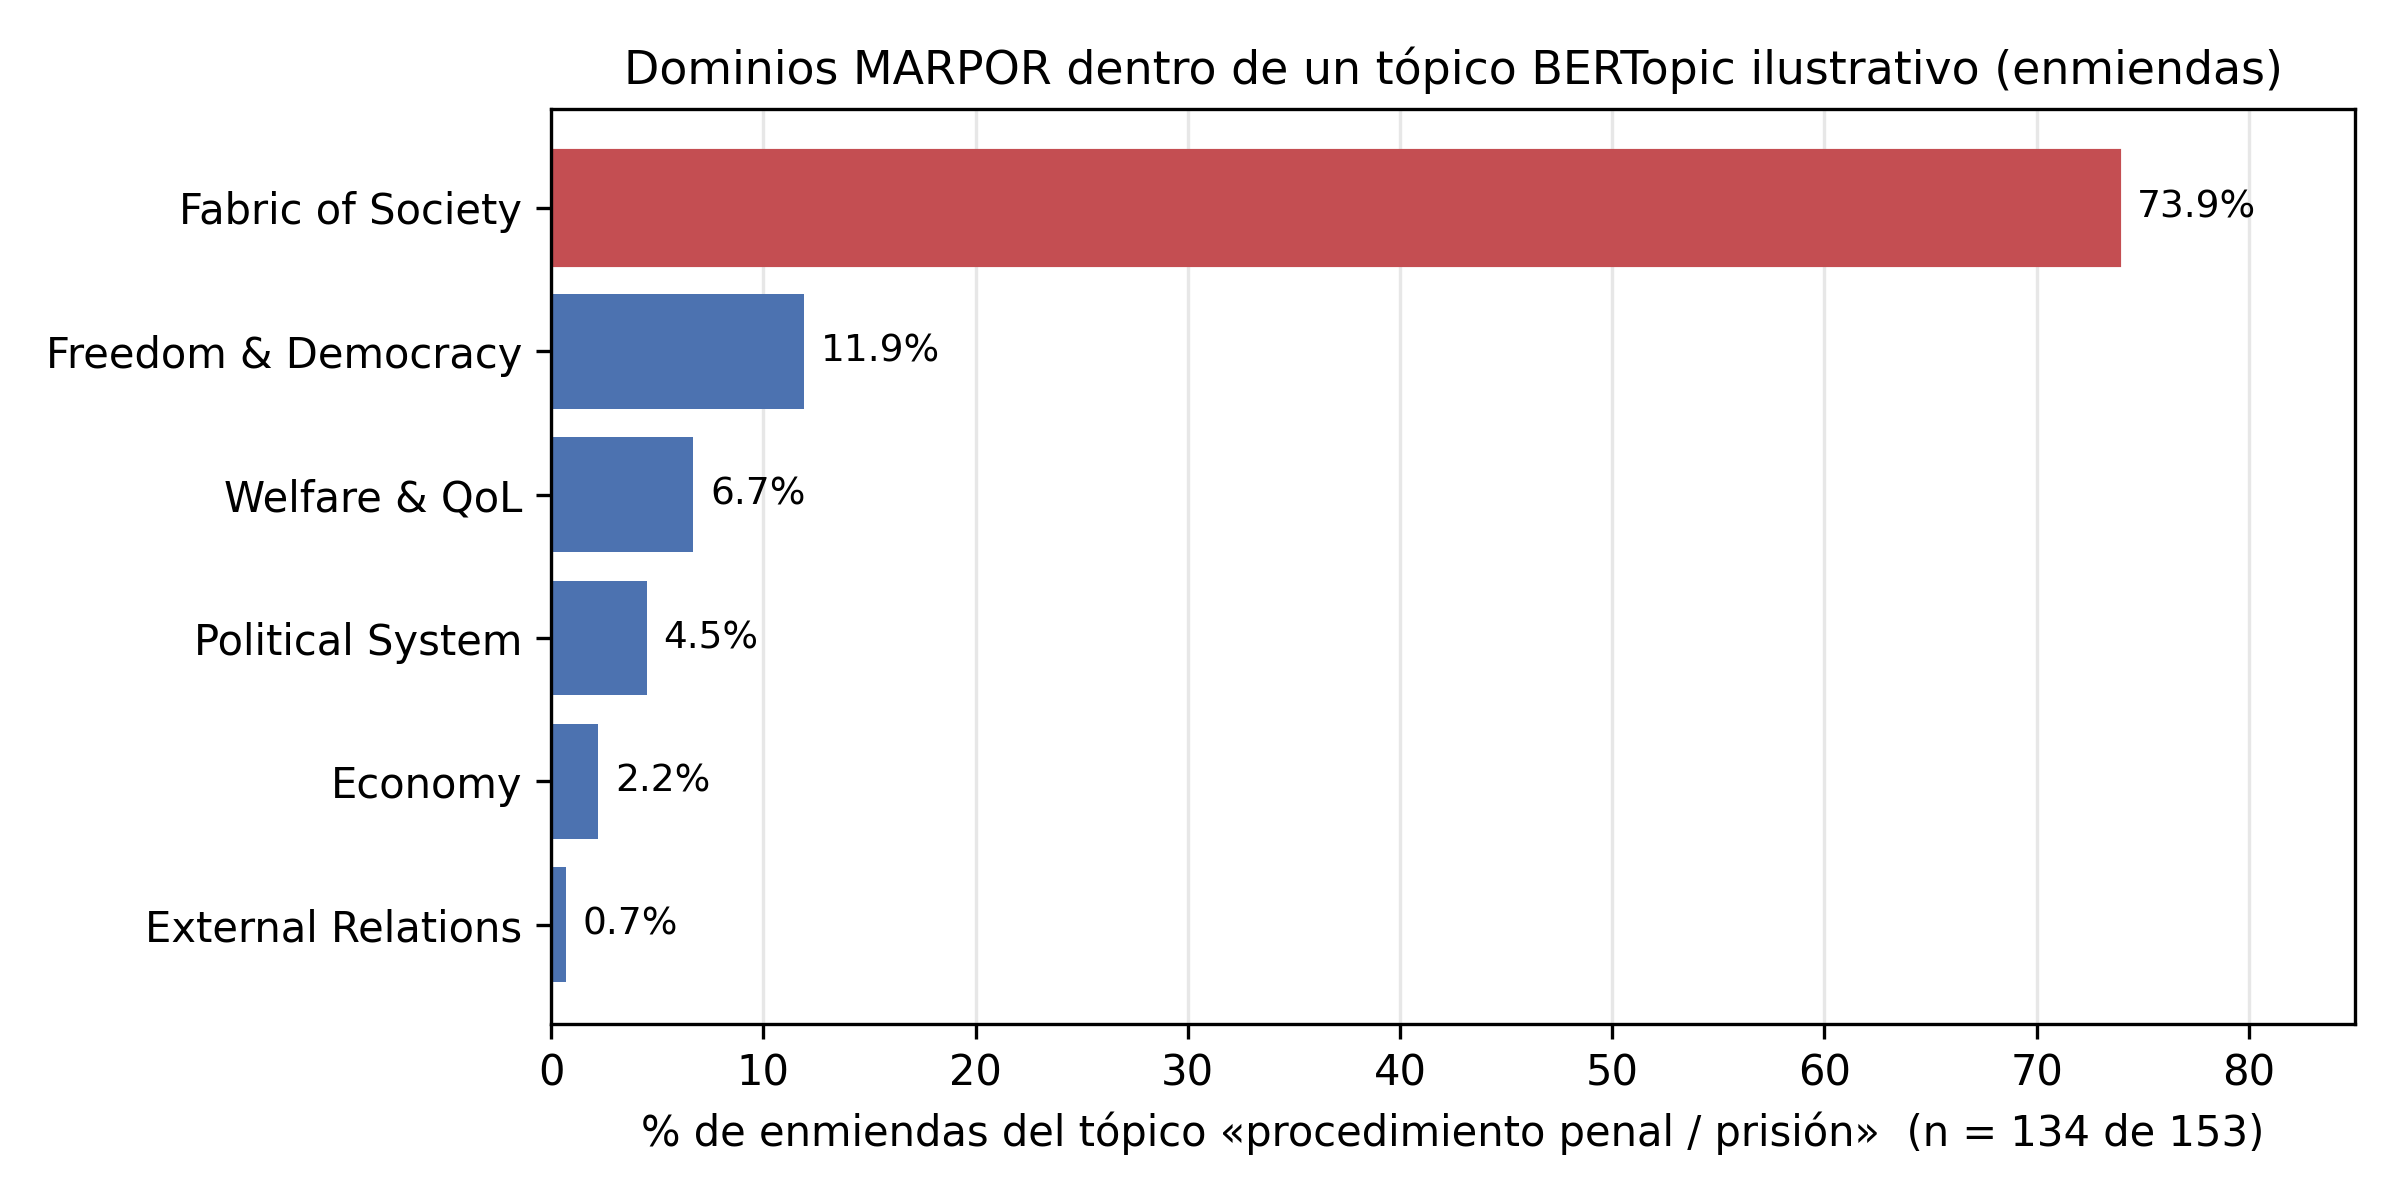
\includegraphics[width=0.85\textwidth]{imagenes/bertopic_marpor_topic_example.png}
  \caption[Cruce ilustrativo BERTopic\,$\times$\,MARPOR]{Distribución de dominios
  MARPOR dentro de un tópico BERTopic ilustrativo: el tópico de enmiendas
  \emph{procedimiento penal / prisión} (134 de 153 documentos enlazados por el
  texto). La figura es ilustrativa y \emph{no} valida un modelo con el otro;
  muestra cómo un agrupamiento empírico no supervisado se distribuye sobre la
  taxonomía supervisada usada en el análisis principal. El enlace se hace por un
  prefijo del texto, por lo que la cobertura es parcial (véase el detalle en el
  cuerpo del anexo).}
  \label{fig:bertopic-marpor}
\end{figure}
